% !TEX root=/home/tavant/these/manuscript/src/manuscript.tex



\section*{Propulsion system for spacecrafts}
\label{sec-propulsion}


In order to evolves in space, satellites, scientific probes and spacecrafts in general rely on a propulsion system.
The cost to go from one planet (usually the Earth) to another location can be expressed as \emph{ Delta-V}, a measure of impulse needed to perform a manoeuvre.
\Cref{fig-subway_DV} illustrates the Delta-V needed to evolve in the solar system.
\begin{figure}[hbtp]
  \centering
  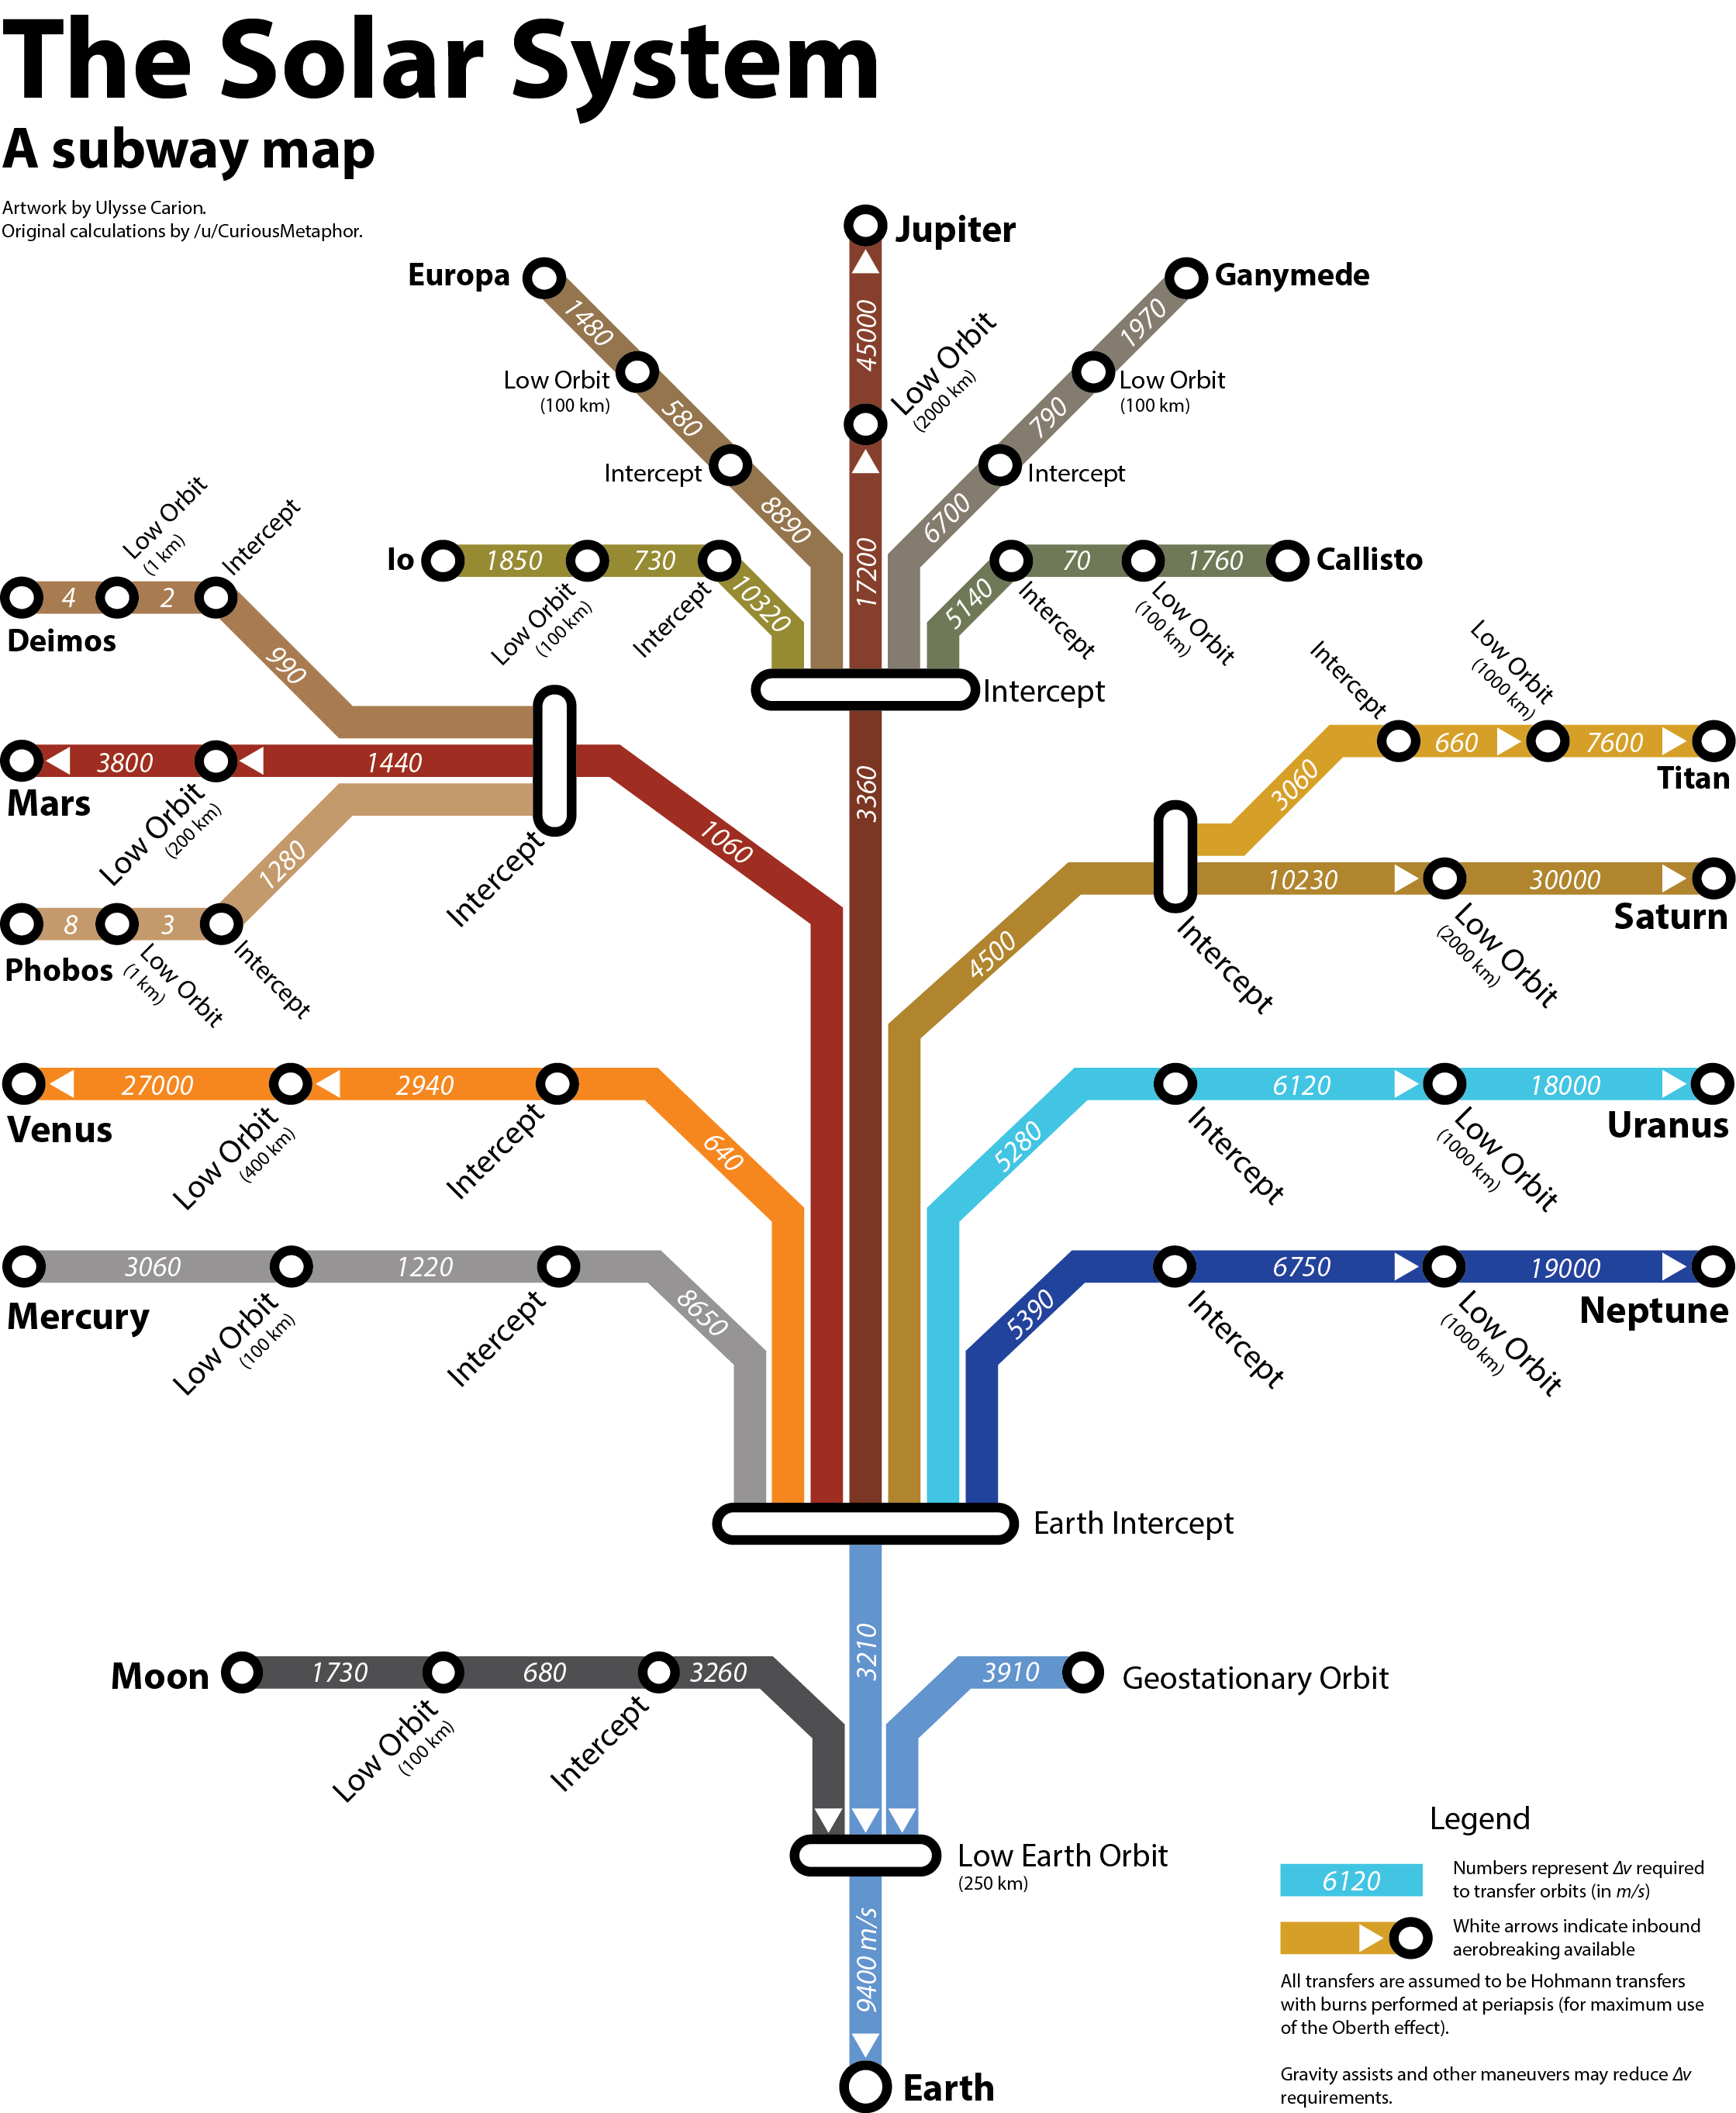
\includegraphics[width=\textwidth]{subway_map}
  \caption{Representation of the different Delta-V needed to go around the solar system, from \citet{reddit-subway}}
  \label{fig-subway_DV}
\end{figure}


For a spacecraft of instantaneous mass $M(t)$, with a propulsion system generating an instantaneous thrust $T(t)$, the Delta-V between $t_1$ and $t_2$ is
\begin{equation} \label{eq-dv}
  \text{Delta-V} = \int_{t_1}^{t_2} \frac{ \norm{T(t)}}{M(t)} dt.
\end{equation}
We see from \cref{eq-dv} that for a more massive spacecraft, a more intense, or a longer thrust is needed in order to obtain the same Delta-V.

\subsection*{Rocket equation}
The thrust $T$ generated by ejecting mass at high velocity is
\begin{equation} \label{eq-thurst}
  T = v_{\rm ex} \dot{M}
\end{equation}
with $v_{\rm ex}$ the exhaust velocity of the propellant, and $\dot{M}$ is the propellant mass flow rate through the thruster.
Hence,
\begin{equation} \label{eq-rocket}
  \text{Delta-V} = \int_{t_1}^{t_2} v_{\rm ex} \frac{ \norm{\dot{M}}}{M(t)} dt = v_{\rm ex} \ln \lp \frac{M_0}{M_1} \rp
\end{equation}
with $M_0 = M(t_0)$ and $M_1=M(t_1)$, and supposing that $v_{\rm ex}$ is constant.
We see from \cref{eq-rocket} that for a given mass $M_1$ to be set to a position after a given Delta-V, the exhaust velocity is a directly link to the initial mass $M_0$.
We usually refer to $M_1$ to the dry mass, and $M_0$ to the wet mass (dry mass plus propellant).
\Cref{eq-rocket} is named the (Tsiolkovsky) rocket equation, 
The exhaust velocity $v_{\rm ex}$ is usually refereed instead by the specific impulse $\Isp = g_0 v_{\rm ex}$, with $g_0$ the standard gravity.
\nomenclature[Q]{\ensuremath{ \Isp}}{ Specific impulse, related to the exhaust velocity of a propellant}
\nomenclature[P]{\ensuremath{ g_0}}{  Standard gravity \nomunit{9.80665 m/s$^2$}}

\subsection*{Chemical and electrical space propulsion systems}
The usual thruster for rocket thruster uses chemical reaction to generate the thrust.
For instance, the Vulcain ( the thruster engine of the main stage of the European Ariane 5 and 6, developed by ArianeGroup, ex Safran) uses the oxygen-hydrogen combustion, the most efficient chemical reaction \citep{nasa-H2O2}
\begin{equation*}
  2 {\rm H_2} + { \rm O_2} = 2 {\rm H_2 O} + 572 \text{~kJ},
\end{equation*}
with the energy of 572~kJ corresponding to 1~mole of oxygen.
This means that burning 1~kg of hydrogen-oxygen mixture deliver an energy of 13~MJ. 

Supposing that of that energy is converted into the exhaust of the water produced, its velocity would be of 5.1~km/s.
In reality, the exhaust velocity of the Vulcain is of 4.2~km/s, corresponding to $\Isp=431$~s.

The fact that the energy source is linked to the propellant mass gives an upper limit of exhaust velocity for a given combustion.
Electrical propulsion engines, on the other hand, decouple the mass ejected (the propellant) from the energy source.
This allows theoretically an unlimited exhaust velocity.
Another advantage is the absence of reactive species, which lowers the security requirements impacting the spacecraft.

\subsection*{Electric propulsion} \label{subsec-label}
\ac{EP} systems mostly rely on plasma \citep{charles2009,mazouffre2016}.
They have been successfully used since the 1960s by governments, but their complexity, the limited electric power available, and the natural risk aversion of the space industry kept the \ac{EP} technologies hidden from the commercial applications \citep{lev2019}.
The breakthrough came in the '90s when the former Soviet Union's companies licenses the technology to western propulsion companies.
However, many commercial satellite manufacturers were sceptical, until the first decade of the 20th century, which brought strong evidences of \ac{EP}.
The landmark of commercial use of \ac{EP} is the selling of 4 all-electric satellites for Geostationary Earth orbit by Boing in 2012, the first 2 of which launched in Marsh 2015.

The two main \ac{EP} technologies used are
\begin{itemize}
  \item the \ac{HET}s, also known as Stationary Plasma Thruster (SPT) in Russia
  \item the Gridded Ion Thrusters (GIT), usually refereed as Ion Thrusters
\end{itemize}

Recently, the first satellites of two mega-constellations (OneWeb, 648 satellites, from which 6 were launched on February, the \nth{26} 2019, and Startlink, 12,000 satellites, from which 62 were launched on May, \nth{23} 2019) were send two Low Earth orbit, both using Hall effect thrusters. 


 
 \paragraph{The Gridded Ion Thruster} is a plasma chamber closed at one end by two or more grids.
 The plasma source is an emitting cathode, generating energetic electrons that ionize the propellant, usually Xenon.
 The ions are accelerated by the potential difference between the grids.
 Another cathode is used to neutralize the ion beam.
 Compared to \ac{HET}s, it produces an ion beam with less divergence and an higher \Isp of the order of 3000 to 4000~s.
 \Cref{fig-iongridded} shows a picture of the ion thruster used for the BepiColombo mission toward Mercury.
 We clearly see the neutralizing cathode, the accelerating grid and the ion beam.
 
\begin{figure}[hbtp]
  \centering
  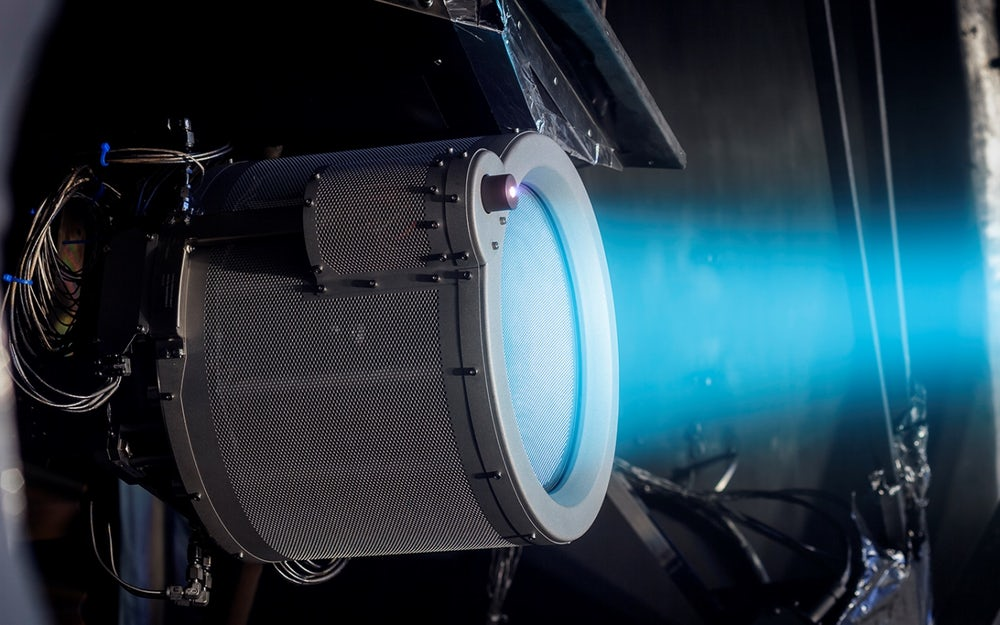
\includegraphics[width=\defaultwidth]{ion_Bepi}
  \caption{The T6 ion thruster will help send BepiColombo to Mercury (Credit: QiniteQ)}
  \label{fig-iongridded}
\end{figure}
 
 \paragraph{Hall Effect thrusters} uses a magnetic barrier to keep the electrons on an annular trajectory, both increasing the ionization of the propellant and creating the accelerating electric field.
 A detailed description of the \ac{HET} is presented in the next section.
 One cathode is used to start the discharge and neutralize the beam.
 Compared to GITs, HETs need less power sources, hence reaching better thrust per power ratio and smaller (hence lighter) Power Processing Unit.
 Their typical \Isp is of the order of 1500~s.
 
 \Cref{fig-13kWHET} shows a high power prototype firing.
 We see the emitting cathode at the center, and the ion beam.
 \begin{figure}[hbtp]
   \centering
   \includegraphics[width=\defaultwidth]{HET_x3}
   \caption{A 13 kilowatt \ac{HET} prototype on a testing bench in a vacuum chamber (Credit: NASA).  }
   \label{fig-13kWHET}
 \end{figure}
 
 
 \subsection*{\ac{EP} environment in France} \label{subsec-HET_thruster}
 
 France is a leader country in the aerospace industry in Europe and in the world, with for example Airbus, Thales, Safran and ArianeGroup.
 Unsurprisingly, its ecosystem of electric propulsion is rich.
 The main French thrusters are the PPS series from Safran, with the \PPS1350 (version G at 1.5~kW nominal power, 89~mN of thrust and \Isp of 1650~s, and the version E at 2.7~kW, at 140~mN of thrust and \Isp of 1800s), and the \PPS5000, a high power \ac{HET} at 5~kW, the first models of which has been delivered to Boeing in May 2019.
 A low-power version of the \PPS{}  is currently developed at Safran \citep{vaudolon2018}.

 
 Several initiative concerning the small-sat sector are also undertaken, as for instance the start-ups Exotrail (micro \ac{HET}) and Thrust Me (radio frequency Ion Thruster), or the Electron Cyclotron Resonance Thruster at ONERA.
 
 A research group on plasma propulsion has been studying \ac{HET} since 1996.
 it is composed of the \ac{CNES}, laboratories as ICARE, LAPLACE and LPP, Safran and ONERA \citep{boniface2017}.
 
 This numerous actors, combined with the support of the France and European space agencies, compose a stimulating environment that contributes both to the most mature technologies and the promising \ac{EP} concepts that could disrupt the propulsion sector.
 